\Chapter{Related Work}\label{chapter:related}

In this chapter, I provide a comprehensive review of existing
approaches relevant to multi-view image generation.

The chapter begins by introducing the fundamental task of Novel View
Synthesis (NVS) and its significance. We then delve into traditional
3D reconstruction techniques (Section \ref{sec:3d-reconstruction})
and their inherent limitations, particularly for sparse-input
scenarios, which motivates the exploration of generative methods.
Subsequently, the discussion shifts to the foundational principles of
Deep Generative Models for Image Synthesis, with a focus on diffusion
models (Section \ref{sec:text-to-image}).

Building on this, we explore various methods for Conditioning
Diffusion Models for Enhanced Control and New Tasks (Section
\ref{sec:conditioning-diffusion}), including the crucial role of
camera parameter encoding and the concept of lightweight adaptation
through adapters.

The core of the chapter then examines state-of-the-art
Diffusion-based Multi-View Image Generation techniques (Section
\ref{sec:multi-view-diffusion}), covering both single reference image
novel view synthesis and architectures for coherent multi-view
generation, including specialized multi-view adapters.
%  Finally, the chapter will conclude with a summary of the discussed
% methods and highlight identified research gaps that this thesis
% aims to address.

\section{Traditional 3D Reconstruction Approaches}\label{sec:3d-reconstruction}

Simultaneous Localization and Mapping (SLAM) is a fundamental concept
in the field of computer vision and robotics. It refers to the
process of simultaneously estimating the camera's position and
orientation in a 3D environment while mapping the environment itself.
Originally, SLAM was used to track the position of a robot in a 3D
space, but it has since been applied to a wide range of problems,
including augmented reality, medical applications and novel view
synthesis. To address these requirements, researchers have
concentrated on creating techniques for machines to independently
build ever more precise scene representations. This integration of
robotics, computer vision, sensor technology, and recent advancements
in artificial intelligence has shaped this field.

Typically, SLAM techniques use a combination of data sources, such as
images, laser range scans, sonars and GPS to effectively map an environment.
In this work I will focus on the use of images for 3D reconstruction.

\subsection{From Images to 3D}

One of the most popular methods for 3D reconstruction from images is
COLMAP \cite{colmap}. COLMAP is a general-purpose
structure-from-motion (SfM) \cite{multipleviewgeometry} system that
can automatically reconstruct 3D scenes from a collection of images.
It is a popular choice for 3D reconstruction due to its accuracy,
speed, and ease of use.

\begin{figure}[h]
  \centering
  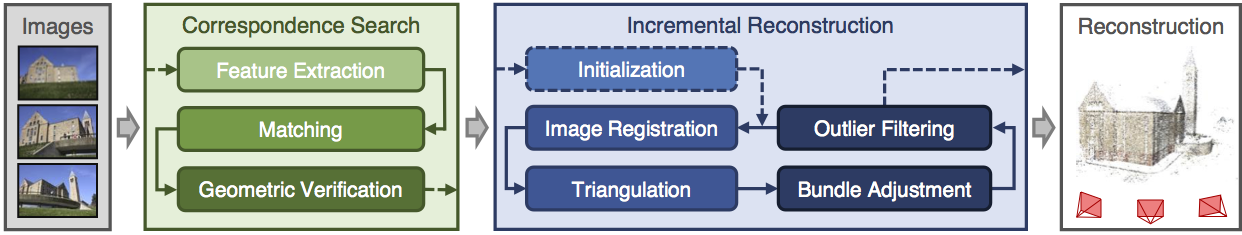
\includegraphics[width=0.9\textwidth]{images/related-work/COLMAP.png}
  \caption{COLMAP pipeline}
  \label{fig:colmap-pipeline}
  % https://colmap.github.io/tutorial.html
\end{figure}

Structure from Motion works in two main steps [Figure
\ref{fig:colmap-pipeline}]:
\begin{enumerate}
  \item \textbf{Correspondence Search}: Identify the unique landmarks
    (features) in all of the images and match the same landmarks across images.
  \item \textbf{Incremental Reconstruction}: Estimates the camera
    poses and triangulates 3D points through an iterative process.
\end{enumerate}

First step of correspondence search is feature extraction. COLMAP
uses SIFT \cite{sift} and ORB \cite{orb} methods to extract features
from images. Scale-invariant feature transform (SIFT) is a method for
detecting keypoints that contrast with their surroundings and
describing the local image content around them. It is invariant to
rotation and scale, can detect keypoints in a number of resolutions
and orientations. Oriented FAST and Rotated BRIEF (ORB) is a more
computationally efficient alternative to SIFT, combining a high-speed
FAST detector with a number of optimizations for rotation resistance,
offering good performance with much less computational load.

\begin{figure}[h]
  \centering
  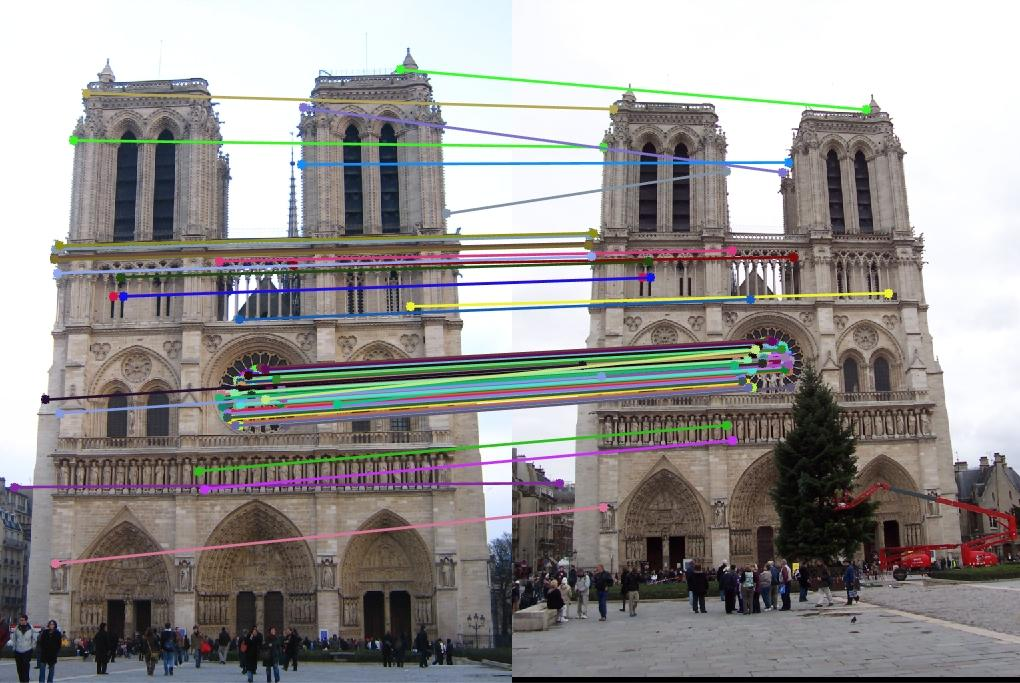
\includegraphics[width=0.7\textwidth]{images/related-work/feature-matching.jpg}
  \caption{Feature matching result}
  \label{fig:matching-features}
  % https://blog.roboflow.com/image-matching/
\end{figure}

Second step is matching features across images. Feature matching is a
process of finding the best matches of features across the images.
COLMAP uses a variant of the FLANN \cite{flann} library to find the
best matches for each feature. FLANN is a library for performing fast
approximate nearest neighbor searches in high dimensional spaces.
Feature matching is visualized in Figure \ref{fig:matching-features}.

Then the geometric verification step uses the prior knowledge about
the camera model and motion to remove outliers, preparing the
verified feature matches for the subsequent Incremental Reconstruction phase.

When it comes to Incremental Reconstruction, the process is as follows:
\begin{enumerate}
  \item \textbf{Camera Pose Estimation}: Estimate the camera location
    and direction in 3D space for each image.
  \item \textbf{Triangulation}: Triangulate 3D points of the observed
    objects from the camera poses and matched features.
  \item \textbf{Bundle Adjustment}: Refine the camera poses and 3D
    points to minimize the reprojection error.
\end{enumerate}

\begin{figure}[h]
  \centering
  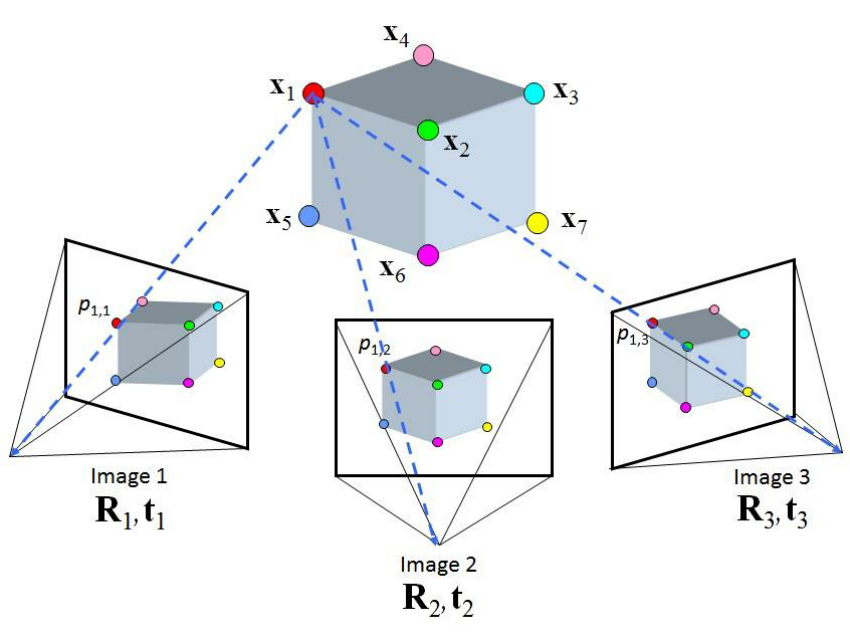
\includegraphics[width=0.5\textwidth]{images/related-work/Structure-from-Motion-SfM-process-is-illustrated-The-structure-in-the.png}
  \caption{Structure from Motion process}
  \label{fig:structure-from-motion}
  % https://www.researchgate.net/figure/Structure-from-Motion-SfM-process-is-illustrated-The-structure-in-the_fig2_269327935
\end{figure}

\begin{figure}[h]
  \centering
  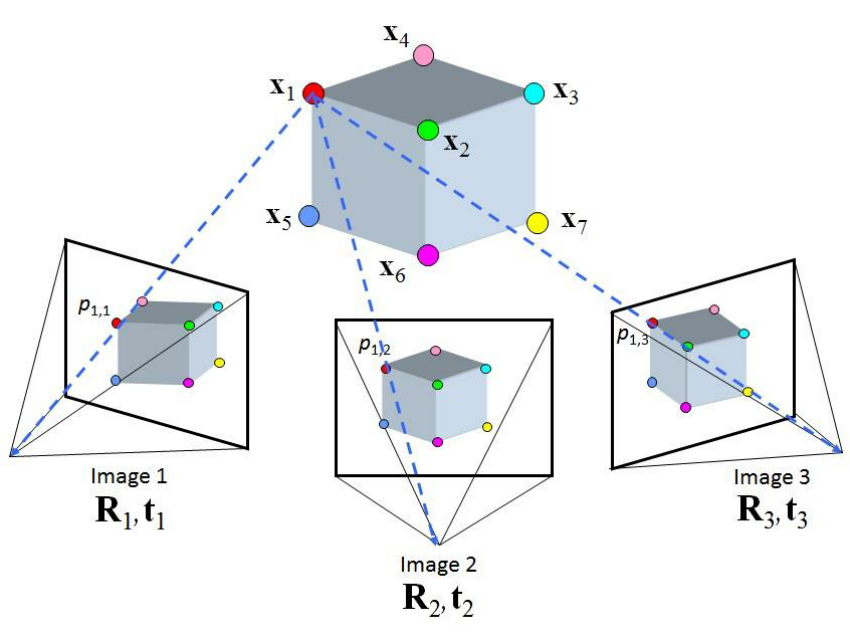
\includegraphics[width=0.5\textwidth]{images/related-work/Structure-from-Motion-SfM-process-is-illustrated-The-structure-in-the.png}
  \caption{Camera pose estimation}
  \label{fig:camera-pose-estimation}
  % https://www.researchgate.net/figure/Structure-from-Motion-SfM-process-is-illustrated-The-structure-in-the_fig2_269327935
\end{figure}

The camera pose estimation (visualized in Figure
\ref{fig:camera-pose-estimation}) starts with an initialization step,
where the initial pair of images and matched features between them
are used to estimate the camera pose. Then, the algorithm proceeds to
the loop (Figure \ref{fig:colmap-pipeline}), where the next image is
registered to the reconstruction and the camera pose is estimated
again (triangulation step). After that the bundle adjustment step is
performed to refine the camera poses and 3D points to be consistent
with the entire dataset with images of a given scene. This
optimization process typically uses the Levenberg-Marquardt algorithm
to minimize reprojection error. This process is repeated for each
subsequent batch of images, updating the camera poses and 3D points.

\subsection{Methods for 3D Reconstruction}

% \subsection{Generative 3D Reconstruction
% Methods}\label{sec:generative-3d-reconstruction}

\subsection{Limitations of 3D Reconstruction}

Structure from Motion is a powerful tool for 3D reconstruction,
demonstrating high effectiveness across a variety of scenarios.
However, it encounters significant challenges when dealing with
textureless surfaces, reflective materials, the computational
complexity of processing high resolution images and most importantly
in context of my work, sparse input scenarios, such as those
involving a single image or only a few images.

% \subsection{Motivation for Novel View
% Synthesis}\label{sec:novel-view-synthesis}

\section{Deep Generative Models for Image Synthesis}\label{sec:text-to-image}

The emergence of powerful diffusion models has revolutionized the
field of image generation, including novel view synthesis. These
models have demonstrated remarkable capabilities in generating
high-quality images conditioned on various inputs, such as text
prompts, reference images, or camera poses.

\subsection{Diffusion Models}

UNET

\subsection{Text-to-Image Diffusion Models}

Text-to-image diffusion models like Stable Diffusion
\cite{stablediffusion} have shown impressive capabilities in
generating diverse and high-quality images from textual descriptions.
Building upon these foundations, several works have extended these
models to handle image-to-image translation tasks, where a reference
image serves as an additional conditioning signal.

\section{Conditioning Diffusion Models for Enhanced Control and New
Tasks}\label{sec:conditioning-diffusion}

\subsection{Diverse Conditioning Signals}

\subsection{Camera Parameter Encoding for 3D Awareness}

\subsection{Lightweight Adaptation}

To address the limitations of full fine-tuning approaches, recent
works have explored adapter-based methods that allow for more
efficient adaptation of pre-trained models to specific tasks while
preserving their original capabilities.

Adapters are lightweight modules that can be inserted into
pre-trained models to adapt them to new tasks without modifying the
original network parameters. This approach has gained popularity in
natural language processing and has also been applied to diffusion
models for various image generation tasks.

ControlNet \cite{controlnet} introduced a method to add spatial
conditioning to text-to-image diffusion models by training additional
control modules that are connected to the original UNet backbone.
This approach allows for precise control over the generated images
while preserving the original model's capabilities.

Similarly, T2I-Adapter \cite{t2iadapter} proposed a more modular
approach where adapters are trained separately and can be combined to
provide multiple forms of control simultaneously. These methods have
demonstrated the effectiveness of adapter-based approaches for
controlled image generation.

\section{Diffusion-based Multi-View Image
Generation}\label{sec:multi-view-diffusion}

\subsection{Single Reference Image Novel View Synthesis}

Zero-1-to-3 \cite{zero1to3} pioneered the approach of conditioning
diffusion models on both a reference image and camera pose
information to generate novel views. This method demonstrated the
potential of leveraging pre-trained text-to-image models for novel
view synthesis without requiring explicit 3D reconstruction. However,
it often struggles with maintaining geometric consistency across
generated views.

\subsection{Coherent Multi-View Generation Architectures}
% Camera encoding

To address the limitations of single-view approaches, several works
have focused on developing multi-view diffusion models that can
generate multiple consistent views simultaneously.

MVDream \cite{mvdream} extends the self-attention mechanism in
diffusion models to operate across multiple views, enabling the
generation of 3D-consistent images. By jointly modeling multiple
views, this approach significantly improves geometric consistency
compared to methods that generate each view independently.

Similarly, ViewCrafter \cite{viewcrafter} combines video latent
diffusion models \cite{videolatentdiffusion} with 3D point cloud
priors to generate high-fidelity and consistent novel views. By
leveraging the explicit 3D information provided by point clouds and
the generative capabilities of video diffusion models, ViewCrafter
achieves precise control of camera poses and generates high-quality novel views.

CAT3D \cite{cat3d} takes a different approach by simulating a
real-world capture process with a multi-view diffusion model. Given
one or three input images and a set of target novel viewpoints, this
model generates highly consistent novel views that can be used as
input to robust 3D reconstruction techniques.

While these multi-view diffusion models have shown impressive
results, they typically require full fine-tuning of pre-trained
text-to-image models, which is computationally expensive and may lead
to degradation in image quality due to the scarcity of high-quality 3D data.

\subsection{Specialized Multi-View Adapters}

Building upon the success of adapter mechanisms, MV-Adapter
\cite{mvadapter} introduced the first adapter-based solution for
multi-view image generation. Unlike previous approaches that make
invasive modifications to pre-trained text-to-image models and
require full fine-tuning, MV-Adapter enhances these models with a
plug-and-play adapter that preserves the original network structure
and feature space.

MV-Adapter employs a decoupled attention mechanism, where the
original spatial self-attention layers are retained, and new
multi-view attention layers are created by duplicating the structure
and weights of the original layers. These layers are organized in a
parallel architecture, allowing the adapter to inherit the powerful
priors of the pre-trained self-attention layers while efficiently
learning geometric knowledge.

Additionally, MV-Adapter introduces a unified condition encoder that
seamlessly integrates camera parameters and geometric information,
facilitating applications such as text and image-based 3D generation
and texturing. By updating fewer parameters, MV-Adapter enables
efficient training and preserves the prior knowledge embedded in
pre-trained models, mitigating overfitting risks.
